\begin{document}
\sectiontitle{10}{Closed-Loop FES Control}
\setstretch{1.6}
\lhead{Closed-Loop FES Control} % section header
The final closed-loop control system was designed and implemented in order to improve the quality of the stimulated step while also minimizing fatigue.  This system dynamically adjusts the stimulation current amplitude using a Proportional-Integral (PI) controller to apply only the necessary current for achieving the desired movement. Due to the absence of a gait phase detection algorithm, the system relies exclusively on feedback from knee angle measurements and uses a time-dependent reference for the knee angle. 

\subsection{Methods}
\lhead{Closed-Loop FES Control - Methods}
\subsubsection{Closed-Loop Design}
The methodology for designing the closed-loop system for functional electrical stimulation (FES) began with an assessment of the available resources and constraints. The most significant limitation was the lack of a gait phase detection algorithm, which necessitated an alternative approach for managing state transitions. In addition, the available hardware included inertial measurement units (IMUs) for feedback, which could provide knee angle estimates but no direct phase detection capability. The design was further informed by extensive research and literature on FES and its application in gait rehabilitation.

Given these constraints, the system was designed to rely on open-loop transitions for changing stimulation states. This decision was made because the system operates in a controlled environment where patients walk at a steady speed on a treadmill. In this setting, the consistent speed makes the implementation of a preset stimulation sequence a valid approach.

The next step involved determining how feedback from the IMUs could be incorporated. Knee angle data from the IMUs was selected as the primary variable for controlling the intensity of muscle stimulation. A linear controller was chosen for its simplicity and effectiveness in adjusting stimulation intensity based on real-time knee angle measurements.

The final step was to integrate these elements into an efficient and cohesive control system. This required defining the specific implementations of the key components, including the knee angle reference, gait cycle duration, proportional-integral (PI) controller, feedforward current, and current saturation mechanisms.

\subsubsection{Knee Angle Reference Design}
To use the knee angle error as an input for the PI controller, it is essential to establish a reliable and accurate reference. The first step in the methodology for defining the reference was to consult the literature. However it turned out that seemingly no papers on FES for gait explicitly explain what type of reference they use, although several refer to that they use "well-known" knee angle reference values \cite{bouri_closed-loop_2018}, \cite{ferrante_personalized_2016}, \cite{muller_adaptive_2020}. This is however not very precise since this could be implemented in a myriad of ways. The next step therefore consisted of finding out how to use the typical knee angle values as a reference.

The knee’s range of motion during the gait cycle follows a characteristic pattern. This curve represents the typical knee angle changes that occur during healthy gait and serves as a benchmark for evaluating deviations. A clear example of this pattern is shown in Figure \ref{fig:kneecurvetypical}.

\begin{figure} [h]
    \centering
    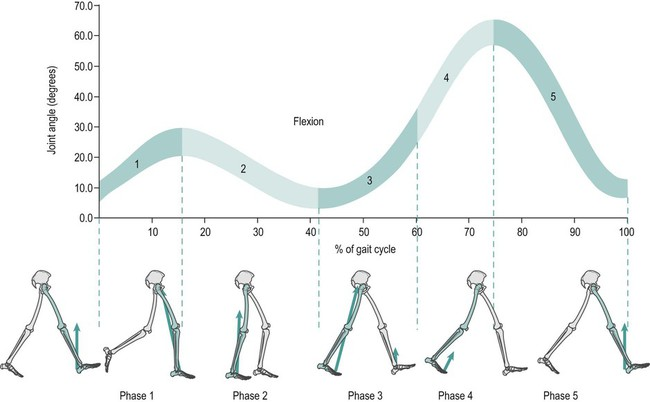
\includegraphics[width=0.99\linewidth]{images/B9780702043444000158_f015-005-9780702043444.jpg}
    \caption{Typical knee angle values during healthy gait \cite{themes_biomechanics_2017}}
    \label{fig:kneecurvetypical}
\end{figure}
It was decided that the knee angle reference would be based on this curve. Instead of implementing static knee angle references for certain phases of the gait cycle, the reference angle would change continuously over time following the reference curve. This decision was made to create smoother transitions and result in more consistent and gradual variations in the stimulation.

Two different approaches to creating the reference curve were attempted. The first involved simply re-creating the general shape and amplitude of the typical knee angle curve by combination of two sinus curves tuned by-hand. 

The second approach involved extracting the curve by fitting a Fourier series to the measured knee angle data during gait. Fourier series fitting is a mathematical method that represents a periodic function as a sum of sine and cosine terms, enabling the decomposition of complex waveforms into simpler harmonic components \cite{blackledget_chapter_2006}. The data for this fitting was sourced from the open-access gait analysis dataset provided by Camargo et al. \cite{camargo_comprehensive_2021}. In this dataset, 20 subjects were equipped with several sensors, including a goniometer attached to the knee, to obtain precise knee angle measurements while walking on a treadmill.

To extract the curve, data from a single dataset recorded at a walking speed of approximately 1 m/s was used. A Fourier series was then applied to approximate the periodic knee angle data. Mathematically, the series is represented as:
\begin{equation}
f(x) = a_0 + \sum_{i=1}^{n} \left( a_i \cos(2\pi i x) + b_i \sin(2\pi i x) \right)
\end{equation}

\begin{itemize}
    \item \(a_0\) is the constant offset (mean value of the function).
    \item \(a_i\) and \(b_i\) are the Fourier coefficients for the cosine and sine terms, respectively.
    \item \(n\) is the number of harmonics, which determines the complexity of the approximation.
\end{itemize}

In order to extract the coefficients that best fit the data the \texttt{curve\_fit} function from \texttt{SciPy} was used. The number of harmonics (\textit{n}) is set to 3 in order to balance accuracy and computational efficiency. This number provides enough flexibility to capture the general shape of the motion without over fitting to noise or adding unnecessary complexity.

\subsubsection{Validation of the Closed-Loop FES Control}
The closed loop implementation was tested on a single healthy subject at two different speeds while walking on the treadmill. The subject attempted to put as little weight on the stimulation leg as possible and relax the muscles during the stimulation sequence to attempt to minimize the affects of voluntary contraction. The subjects leg length was measured and gait cycle duration was set according to the methodology laid out in section on gait cycle duration. After finding the correct electrode placements, the motor and maximum tolerable intensity thresholds were found. The feedforward value was then set to a value between the thresholds and the PI gains were tuned. 
\newpage
\subsection{Closed-Loop Design}
\lhead{Closed-Loop FES Control - Closed-Loop Design}
The selection of the control approach began with an evaluation of various linear control methods, ultimately leading to the choice of a PI controller. A proportional-only controller was deemed insufficient because, while it responds to instantaneous errors, it cannot adequately address steady-state errors. The addition of an integral term, which accumulates error over time, allows the PI controller to effectively compensate for consistent offsets (e.g., under- or over-stimulation) that the proportional term alone cannot eliminate.

In a FES system, delays in muscle activation and mechanical response can cause the actual knee angle to lag behind the desired reference. By including an integral term the controller accounts for these delays indirectly: if the knee angle lags due to delayed muscle response, the accumulated error prompts the system to apply a sustained correction to minimize the offset over time.

The decision to exclude a derivative term was based on its potential impact on system stability. While a derivative term could theoretically improve responsiveness to rapid changes, it would also amplify the noise from IMU measurements and knee angle calculations, risking control loop instability.

\begin{figure} [h]
    \centering
    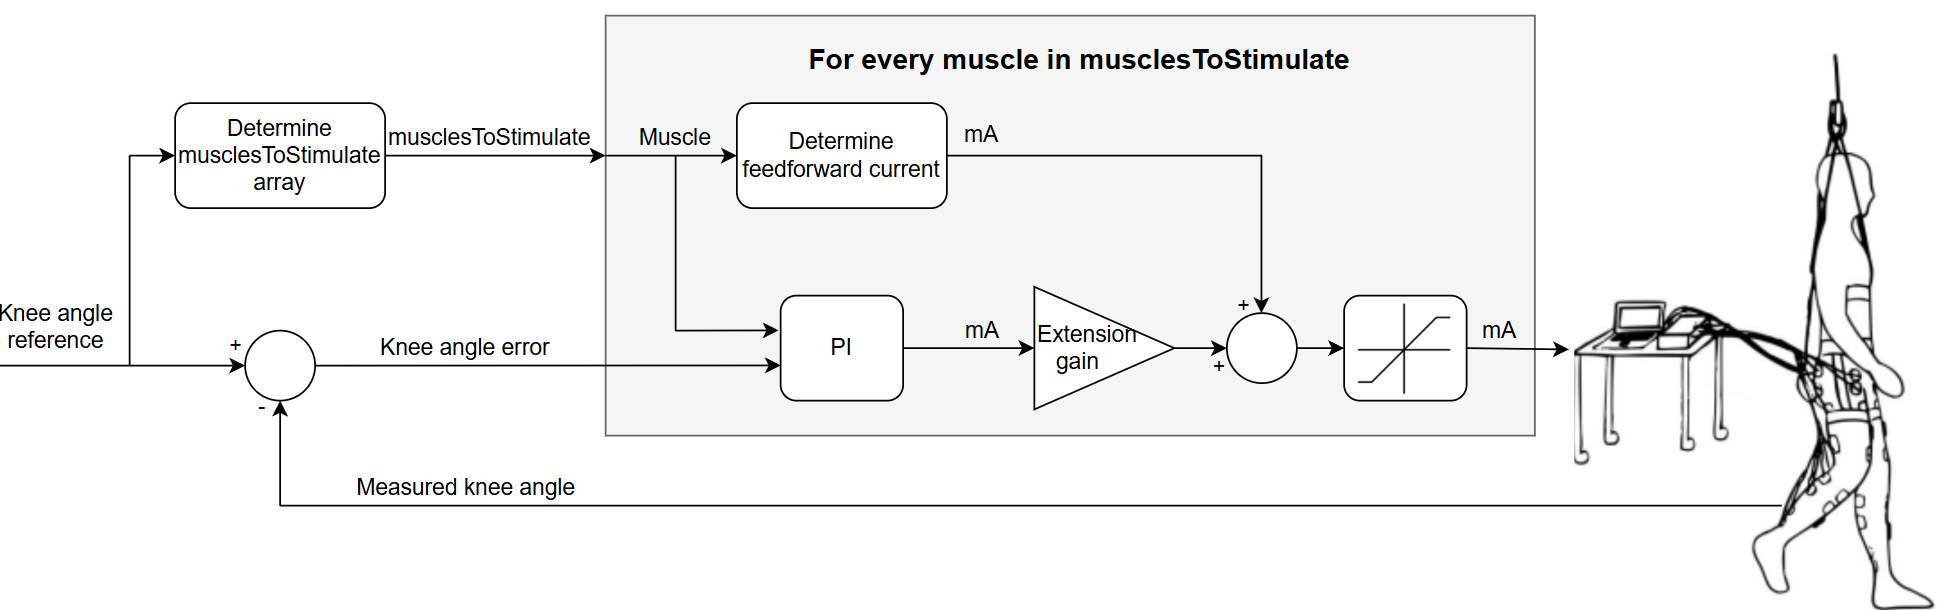
\includegraphics[width=1.1\linewidth]{images/controldiam3.png}
    \caption{Final Closed-loop FES control diagram}
    \label{fig:cldiam}
\end{figure}
\newpage
\begin{wrapfigure}{r}{0.3\textwidth}
    \centering
    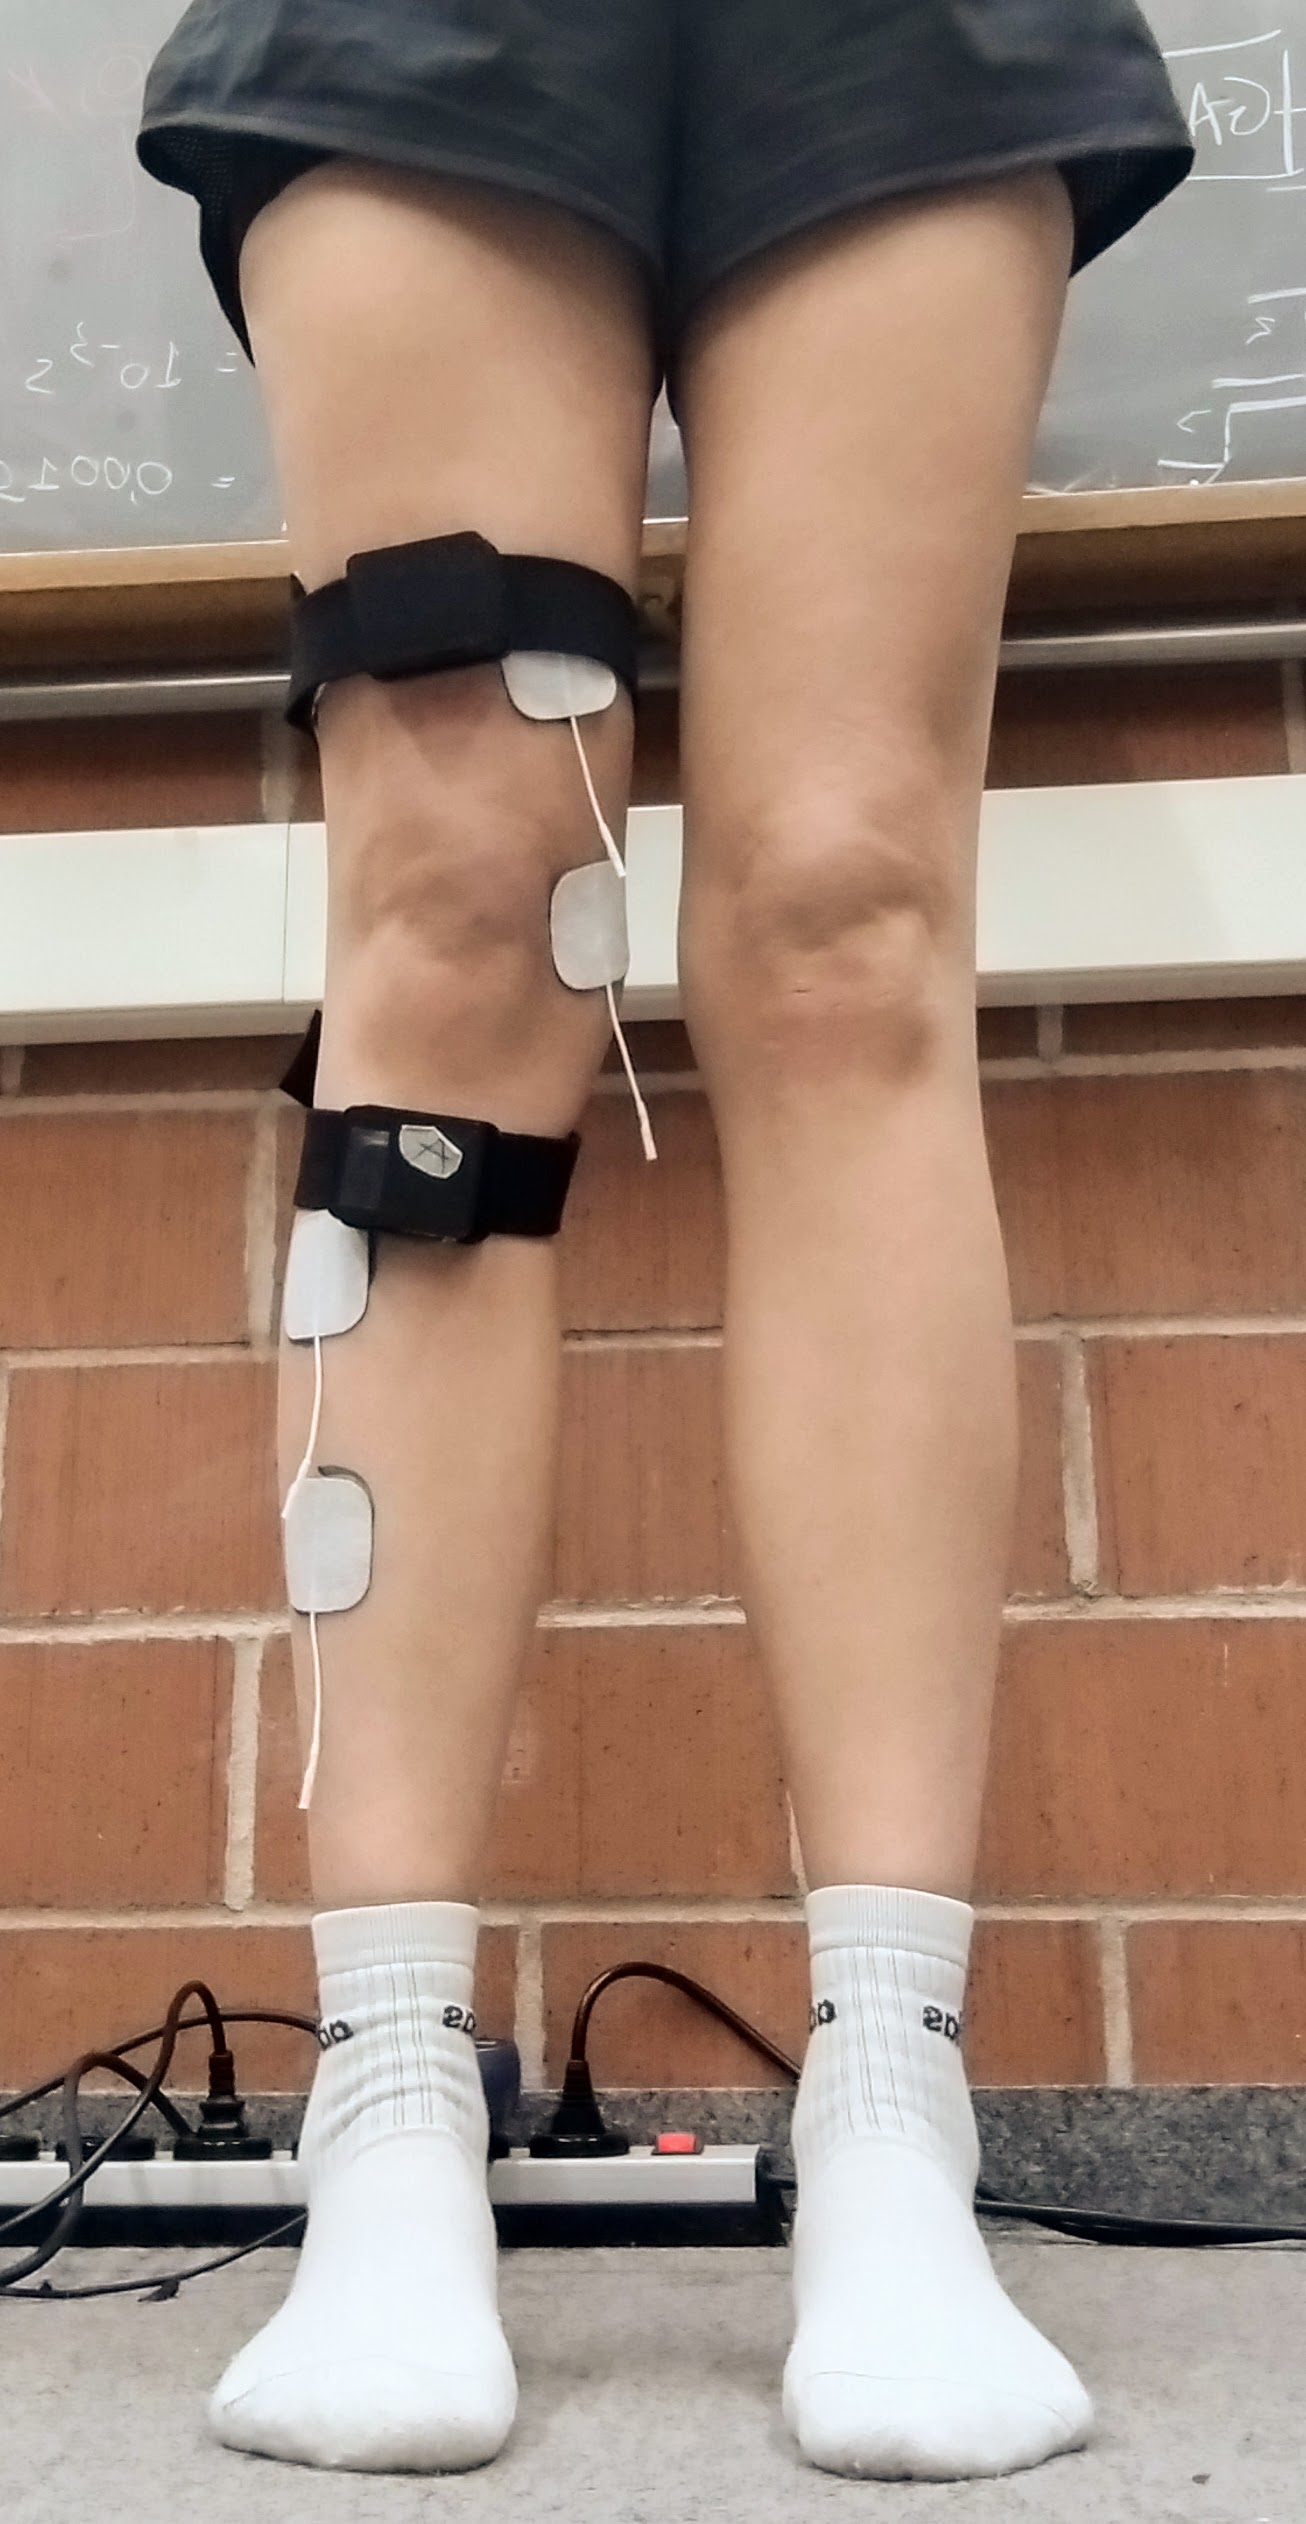
\includegraphics[width=\linewidth]{images/clsetupimg.jpg}
    \caption{IMU and electrode placement for closed loop FES}
    \label{fig:clsetupimg}
\end{wrapfigure}

A visualization of the final design of the closed loop FES control flow can be seen in figure \ref{fig:cldiam}. The system uses a knee angle reference, which is derived from the knee angle reference curve based on the current time and the gait cycle duration. By calculating the current gait cycle percentage, the system determines the corresponding sub-phase of the gait. This information is then used to identify the muscles that need to be stimulated. Where the muscles associated with each sub-phase are based on the open-loop stimulation sequence. 

Then for each muscle that should be stimulated, a PI controller, specifically tuned for that muscle, is executed. Additionally a feed forward current is added to the PI-controlled current and thereafter saturated to determine the final stimulation current. This current is sent to the StimWave board, which delivers the stimulation to the user's muscles via the attached electrodes. The knee angle feedback is obtained fro IMUs placed on the thigh and shank of the leg being stimulated. A picture of the electrode and IMU placements on a single subject can be seen in figure \ref{fig:clsetupimg}.

\subsection{Knee Angle Reference Design}
\lhead{Closed-Loop FES Control - Knee Angle Reference Design}
Two approaches were compared to design the mathematical representation of the knee angle reference curve. First a simple hand-tuned combination of sinusoids, and thereafter a Fourier fitted curve.
\subsubsection{Simplified Curve}
The first mathematical representation of the
The resulting curve from combining two simple sinusoids and hand-tuning parameters is defines as:
\[
y(x) =
\begin{cases}
A_1 \sin\left(2 \pi f_1 x + \phi_1\right) + C_1, & 0 \leq x \leq 40 \\
A_2 \sin\left(2 \pi f_2 x + \phi_2\right) + C_2, & x > 40
\end{cases}
\]
where the parameters are defined as:

For the first bump:
\[
A_1 = 11, \quad f_1 = \frac{0.1}{4}, \quad \phi_1 = \frac{\pi}{2} + 2\pi f_1 \cdot 20, \quad C_1 = 15
\]

For the second bump:
\[
A_2 = 30, \quad f_2 = \frac{0.1}{6}, \quad \phi_2 = -\frac{\pi}{2} + 2\pi f_2 \cdot 80, \quad C_2 = 34
\]
\begin{figure} [H]
    \centering
    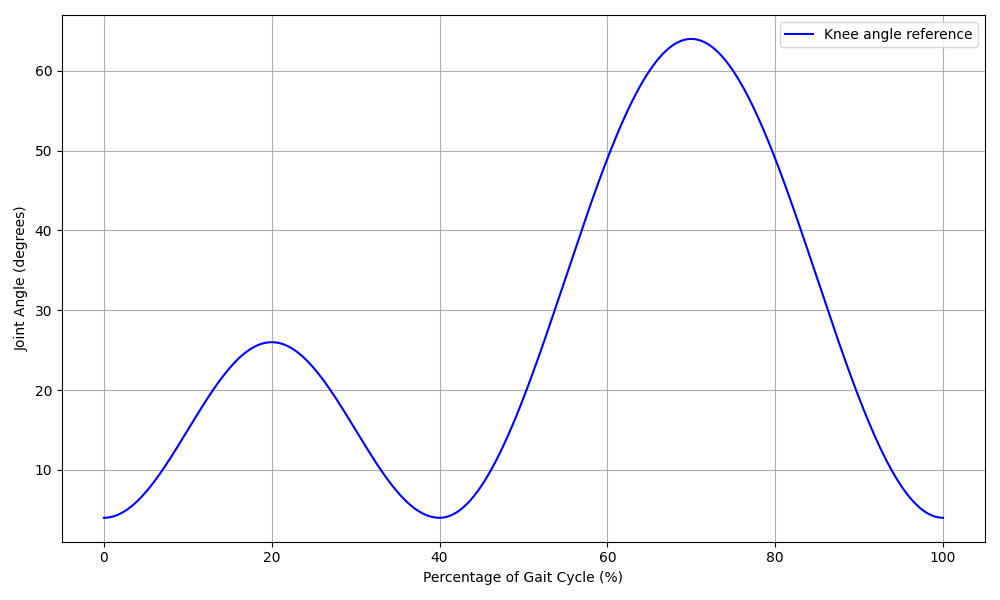
\includegraphics[width=0.8\linewidth]{images/simpleKneeAngle.png}
    \caption{Simplified knee angle curve during gait, created by combining two sinusoids}
    \label{fig:simplecurve}
\end{figure}

A visualization of this curve is shown in Figure \ref{fig:simplecurve}. However, when compared to the typical knee angle curve, significant differences were observed, such as the height of the second sinus curve's peak and the depth of the valley between the two curves.


\subsubsection{Fitted Curve}
The final, more complex, fitted curve is plotted alongside the original data in figure \ref{fig:kneeangleref}, illustrating how well the Fourier series captures the periodic behavior of the knee angle during gait. Its improved resemblance to a physiological knee angle curve, combined with the minimal increase in computational complexity, made it the preferred choice for the closed-loop implementation.
\begin{figure} [H]
    \centering
    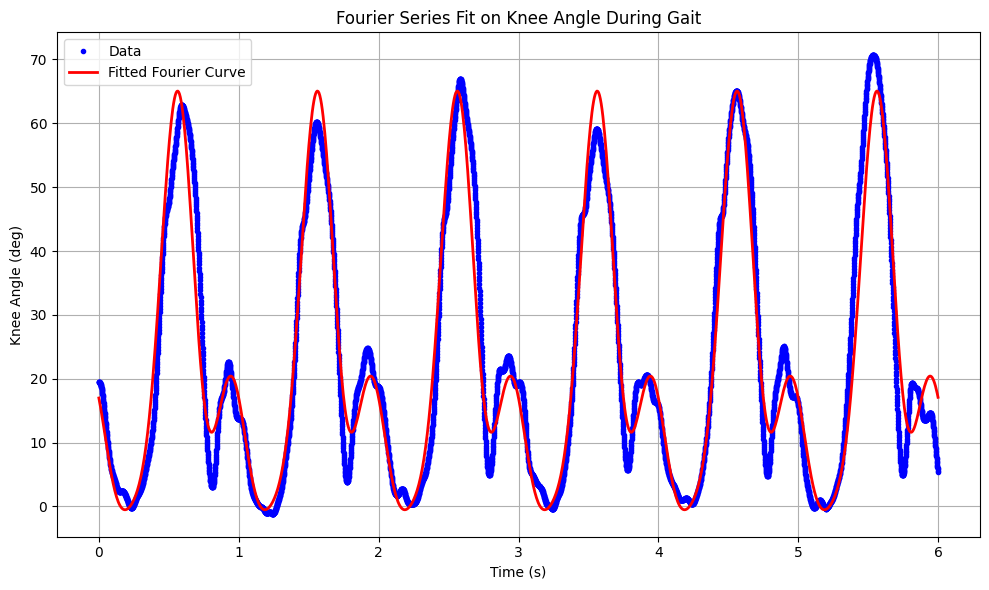
\includegraphics[width=0.99\linewidth]{images/goodkneeangleref.png}
    \caption{Fitted Fourier series curve plotted alongside goniometer knee angle data during gait from \cite{camargo_comprehensive_2021}}
    \label{fig:kneeangleref}
\end{figure}
\begin{figure} [H]
    \centering
    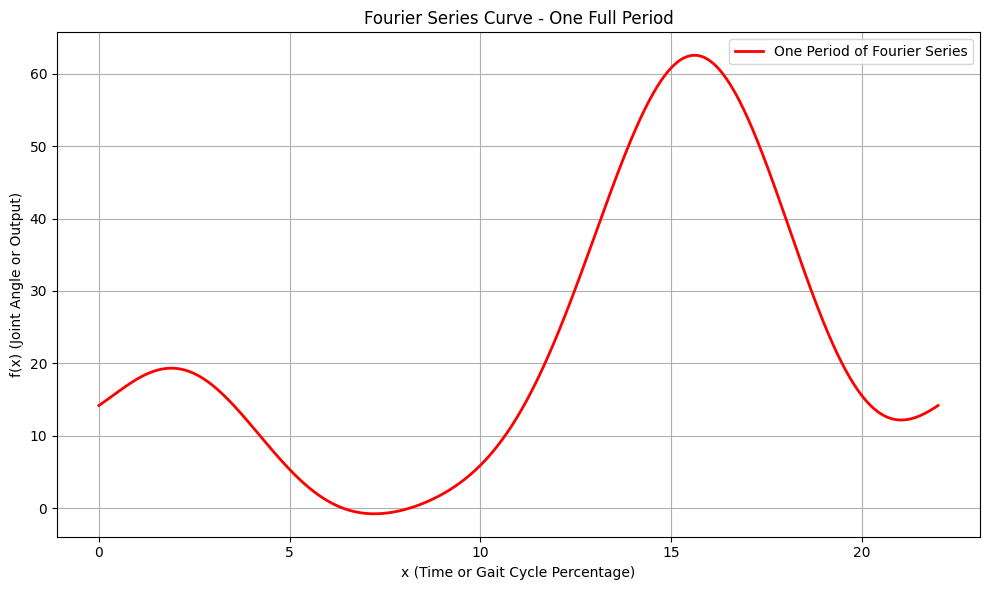
\includegraphics[width=0.85\linewidth]{images/fittedKneeAngleRef.png}
    \caption{Final reference curve, obtained by fitting a Fourier series to knee angle data}
    \label{fig:enter-label}
\end{figure}
\todo{fix figure}


\subsection{Implementation}
\lhead{Closed-Loop FES Control - Implementation}
\subsubsection{Knee Angle Reference}
In order to use the fitted curve as the reference for the PI controller, the knee angle corresponding to the current percentage of the gait cycle must be extracted in real time. This process begins by determining which percentage of the gait cycle the system is currently in. This is calculated using the current time and the gait cycle duration set by the user. The corresponding knee angle is then retrieved from the fitted curve. Which is then fed to the PI controller.

\subsubsection{Gait Cycle Duration}
As mentioned the reference knee angle degree value depends on the gait cycle duration and current time, therefore setting the correct gait cycle duration for each user is an important step. Gait cycle duration defines the time required for one complete stride, encompassing the full sequence of movements from both legs. 

When running the FES experiments on a treadmill this gait cycle duration will vary from user to user and is therefore important to calculate before starting the stimulation. The primary input is the treadmill speed (\(v\)) in (m/s). The second essential parameter is the subjects leg length (\(L\)), measured as the distance from the greater trochanter to the floor in meters \cite{meinders_how_2021}. Then the Froude number (\(Fr)\) which is a widely used descriptor in gait analysis is:
\begin{equation}
    Fr = \frac{v^2}{g \cdot L}
\end{equation}
Where g is gravitational acceleration. Once the Froude number is calculated the stride frequency (\(f_s\)) can be estimated using the following relationship \cite{meinders_how_2021}:
\begin{equation}
    f_s = \sqrt{\frac{g \cdot Fr}{L}}
\end{equation}
From which the gait cycle duration is extracted and inserted into the program to ensure that the closed loop runs on a gait cycle duration that is comfortable for the user.

\subsubsection{PI controller}
To dynamically adjust the current amplitude based on the error between the desired and actual knee angle, a proportional-integral (PI) controller was implemented and tuned for each muscle independently. 

The PI controller was implemented in the \texttt{LoopController} class based on the following discrete time equation:
\begin{equation}
I_{PI}(t) = 
\begin{cases} 
-K_p \cdot e(t) - K_i \cdot \frac{\Delta t}{2} \left(e(t) + e(t-\Delta t)\right), & \text{if extension phase} \\
K_p \cdot e(t) + K_i \cdot \frac{\Delta t}{2} \left(e(t) + e(t-\Delta t)\right), & \text{otherwise}
\end{cases}
\end{equation}

Where \( e(t-\Delta t) \) is the error at the previous time step. As is clear from the formula the integral term is calculated using trapezoidal integration. By averaging the error values at the start and end of the interval the trapezoidal approach better captures the varying nature of the error compared to rectangular integration which assumes that the error remains constant during the interval \(\delta t\). It also reduces the likelihood of abrupt changes to the PI output since it accounts for error trends between time steps rather than using just the current error.

The PI controller also incorporates a phase-specific adaptation. This is because in knee extension increasing the stimulation of the extensor muscles decreases the knee angle, while increased stimulation of flexion muscles will increase the knee angle. To prevent counterproductive stimulation the controller therefor inverts its output during extension.

\subsubsection{Feedforward Current}
A feedforward current is implemented for each muscle individually to provide a baseline stimulation amplitude, ensuring sufficient activation to induce movement. It is set around the midpoint between the motor threshold and the maximum tolerable intensity found for each muscle during setup. 

\begin{figure}
    \centering
    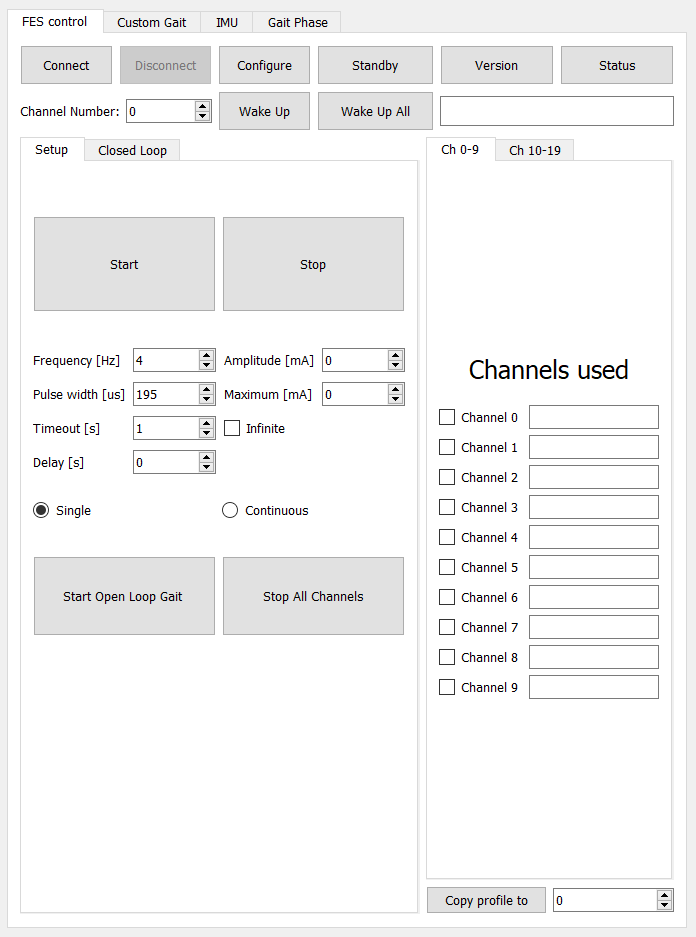
\includegraphics[width=0.65\linewidth]{images/clgui.png}
    \caption{Graphical User Interface for Closed Loop FES, including functionality to tune Kp, Ki, set initial feedforward stimulation and maximum intensity (mA)}
    \label{fig:clsetup}
\end{figure}

Including a feedforward current is particularly beneficial in FES systems because it provides a consistent baseline for muscle activation reducing reliance on reactive feedback adjustments and ensuring smoother, more predictable responses during the gait cycle. It also helps address delays in muscle activation and mechanical response by ensuring timely stimulation even before feedback corrections take effect. Additionally, the feedforward current reduces the workload on the feedback controller by offloading the need for large corrective actions requiring large gain values, allowing the controller to focus on fine-tuning adjustments.

Finally the feedforward current contributes to minimizing muscle fatigue by ensuring that the stimulation is applied more evenly over time. This reduces the need for large corrective currents, which could otherwise lead to over-stimulation and discomfort.

\subsubsection{Current Saturation}
The final calculated current is the sum of the feedforward current and the PI computed current saturated for safety reasons. The maximum possible current amplitude is the maximum tolerable intensity found during the setup and is set for each muscle individually. This saturated current is sent to the StimWave which then applies the stimulation with the set current amplitude, frequency and pulse width to the electrodes for each active muscle.

\subsection{Results}
\lhead{Closed-Loop FES Control - Results}
\subsubsection{Slower Speed}
During the slower speed stimulation the following parameters were tuned and used on the subject:

\begin{table}[h!]
\centering
\caption{Closed Loop Parameters for 0.8km/h}
\begin{tabular}{|l|c|c|c|c|c|}
\hline
\textbf{Muscle} & \textbf{Feedforward Current (mA)} & \textbf{Stimulation Limit (mA)} & \textbf{$K_p$} & \textbf{$K_i$} \\ \hline
Tibialis Anterior  & 35 & 45 & 0.1 & 0.05 \\ \hline
Vastus Medialis    & 25 & 35 & 0.3 & 0.05 \\ \hline
Gastrocnemius      & 35 & 45 & 0.1 & 0.05 \\ \hline
Hamstring          & 35 & 50 & 0.4 & 0.05 \\ \hline
\end{tabular}
\label{tab:closed_loop_9}
\end{table}

\begin{figure} [H]
    \centering
    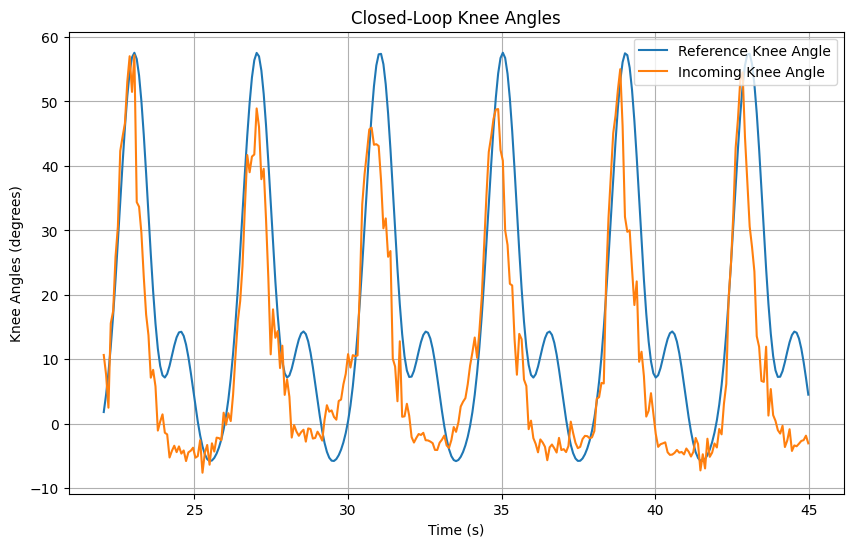
\includegraphics[width=0.95\linewidth]{images/CL9refpng.png}
    \caption{Closed loop knee angles for 0.8km/h}
    \label{fig:cl9ref}
\end{figure}

\begin{figure} [H]
    \centering
    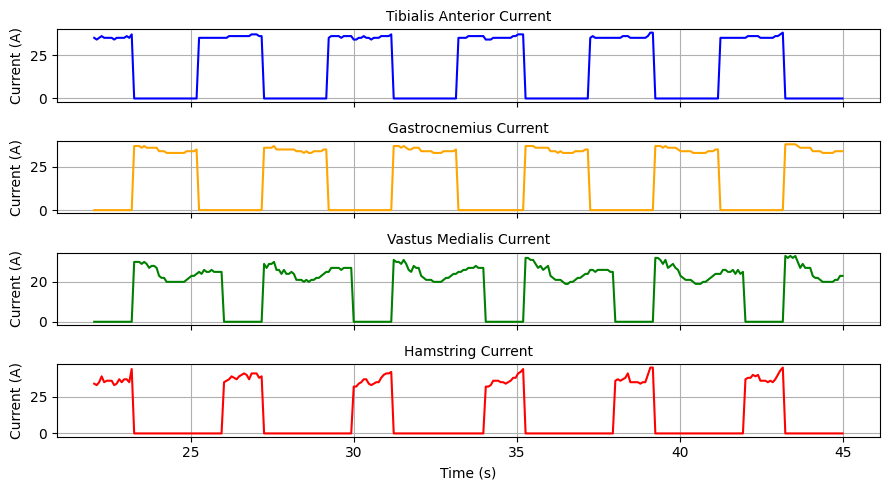
\includegraphics[width=0.9\linewidth]{images/CL9stimpng.png}
    \caption{Closed loop stimulation for 0.8km/h}
    \label{fig:cl9stim}
\end{figure}

Based on the results seen in figure \ref{fig:cl9ref} and \ref{fig:cl9stim}, the closed loop control system demonstrates a reasonable ability to follow the major peaks and valleys of the reference knee angle trajectory at the slower speed of 0.8 km/h. The measured knee angle aligns well with the timing and amplitude of the primary peaks. 

However, the system struggles to replicate the smaller peaks and subtler variations in the reference trajectory. This discrepancy could can be attributed to limitations in the PI controls responsiveness to small variations in reference knee angle and delay in muscle response. This issue might however be possible to mitigate by further tuning of the gains. As can be observed in figure \ref{fig:cl9stim} the variation in stimulation amplitude is not very large, indicating that there is room for increasing the gains and thus the variation in intensity.  

Notably, there is minimal delay observed between the initiation of the initial spike in the reference signal and the corresponding response in the measured knee angle. This highlights the control systems rapid reaction time, which is crucial for maintaining synchronization with the reference gait pattern.

\todo{talk more about the stimulation and compare with open loop stimulation}

\subsubsection{Faster Speed}
During the faster speed (1.5km/h) the following parameters were tuned and used on the subject:

\begin{table}[h!]
\centering
\caption{Closed Loop Parameters for 1.5km/h}
\begin{tabular}{|l|c|c|c|c|c|}
\hline
\textbf{Muscle}  & \textbf{Feedforward Current (mA)} & \textbf{Stimulation Limit (mA)} & \textbf{$K_p$} & \textbf{$K_i$} \\ \hline
Tibialis Anterior & 35 & 45 & 0.2 & 0.05 \\ \hline
Vastus Medialis   & 20 & 35 & 0.4 & 0.05 \\ \hline
Gastrocnemius     & 35 & 45 & 0.2 & 0.05 \\ \hline
Hamstring          & 35 & 50 & 0.5 & 0.05 \\ \hline
\end{tabular}
\label{tab:closed_loop_12}
\end{table}

\begin{figure} [H]
    \centering
    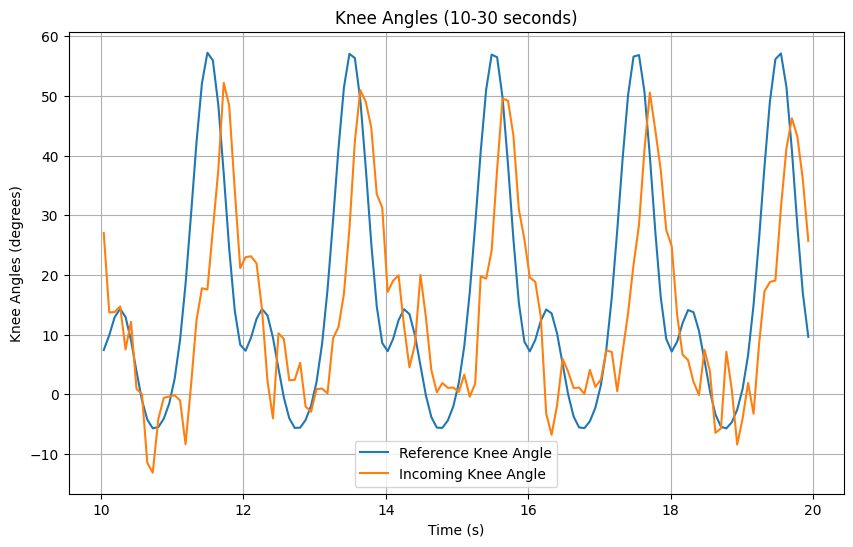
\includegraphics[width=0.9\linewidth]{images/CL12ref.png}
    \caption{Closed loop knee angles for 1.5km/h}
    \label{fig:cl12ref}
\end{figure}

\begin{figure} [H]
    \centering
    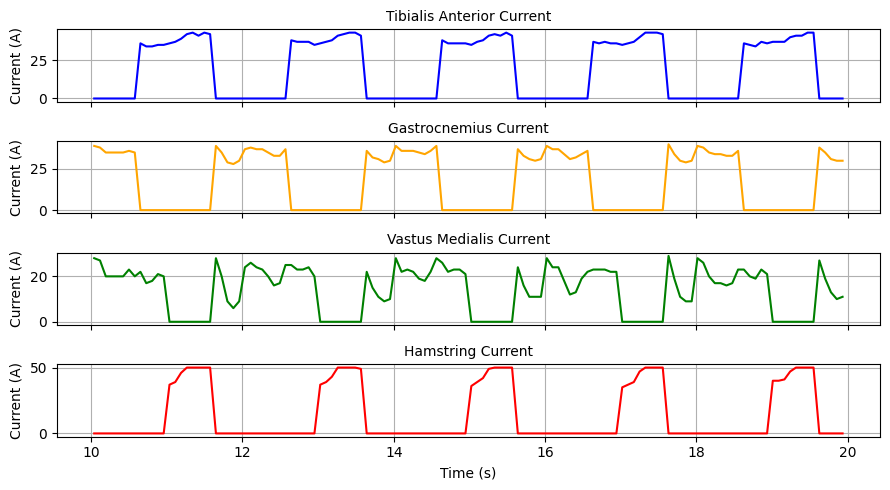
\includegraphics[width=0.9\linewidth]{images/CL12stim.png}
    \caption{Closed loop stimulation}
    \label{fig:cl12stim}
\end{figure}

\todo{Take a look at raw IMU data}
\todo{Take a look at Open loop, compare stim}

At a faster speed of 1.5km/h the results (figure \ref{fig:cl12ref} demonstrate that the closed-loop control system is capable of following the general trajectory of the reference knee angle values. However there is a marked delay between the reference curve and the measured curve, which was not present to the same degree at a slower speed.

Another interesting observation is that the systems seems to more accurately capture the smaller peaks in the trajectory compared to the slower speed. This is likely due to the increased gains in the control system leading to larger variations in the stimulation amplitude as can be seen in figure \ref{fig:cl12stim}.

Compared to the slower speed it is also clear the sampling frequency of the IMU measurements might be becoming an issue at this speed. This is particularly evident during periods of faster transitions, in which the measured signal becomes more jagged and noisy, possibly leading to suboptimal stimulation intensities being applied. 

\subsection{Discussion}
\lhead{Closed-Loop FES Control - Discussion}
The results of the closed-loop gait control system provide an initial insight into the system's capabilities and limitations. The first issue is that of the difficulty of testing FES on healthy subjects, discussed earlier for the Open-Loop stimulation sequence.

The limited subject pool is another issue. Testing on a single subject restricts the generalizability of the results and does not account for individual variability. Differences in muscle composition, skin impedance and motor thresholds could significantly affect the control system's performance. A larger cohort of subjects would provide a more comprehensive understanding of the system's robustness.

Finally the delay and jagged IMU signal at faster speeds might indicate the limits of the system's control bandwidth at higher walking speeds. If the IMU signals do not manage to have a high enough accuracy to accurately measure the knee angle the closed loop control will introduce errors into the system that will make it in effect worse than the open loop implementation. The Madgwick filter has been proved to introduce very minimal delays, so this might indicate that the IMU sampling frequency might be insufficient to capture rapid movements accurately. 

\subsubsection*{Choice of Linear Controller}
Different forms of linear controller could have been implemented, ultimately the PI controller was chosen. 
The PI controller selected to for its ability to meet the specific requirements of the system.  Even though the reference angle changes over time a proportional-only controller may not adequately address persistent and steady-state errors as it only responds to the instantaneous error. Adding the integral term which accumulates error over time, effectively compensates for any consistent offset (e.g. under- or over-stimulation) that the proportional term cannot eliminate. 

In a FES system, delays in muscle activation and mechanical response can cause the actual knee angle to lag behind the desired reference. By including an integral term the controller accounts for these delays indirectly: if the knee angle lags due to delayed muscle response, the accumulated error prompts the system to apply a sustained correction to minimize the offset over time.

The justification for not including a derivative term is that even though the derivative term would in theory enhance the responsiveness to rapid changes it would also simplify the noise in the system. The IMU measurements and subsequent knee angle calculation is noisy and including a derivative term could quickly destabilize the control loop.

\subsection{Further Work}
\lhead{Closed-Loop FES Control - Further Work}
Future studies would benefit from adding a weight support system to minimize voluntary recruitment when testing in healthy individuals. However testing in a in individuals with neurological impairments would clearly be the best case scenario. The limited subject pool should be addressed in future work.

In further iterations it would be interesting to use a reference curve that was averaged across multiple subjects in order to make it more generalizable. Possibly making curves based on demographic groups and speed groups such as female young adult or male middle aged, since there is some variation in gait dynamics between demographics, especially related to age and sex and weight.

\end{document}